\chapter{Examples}
\section{Bulk} 
For an example copy from \verb=$TINIBA/examples/surface/nospin/gaas=:\\
\verb=setUpAbinit_gaas.in= and \verb=gaas.xyz=. This is a
bulk GaAs crystal. See results in \verb=gaas/res= and Fig.~\ref{shg-bulk}.
\begin{figure}[h]
\begin{center}
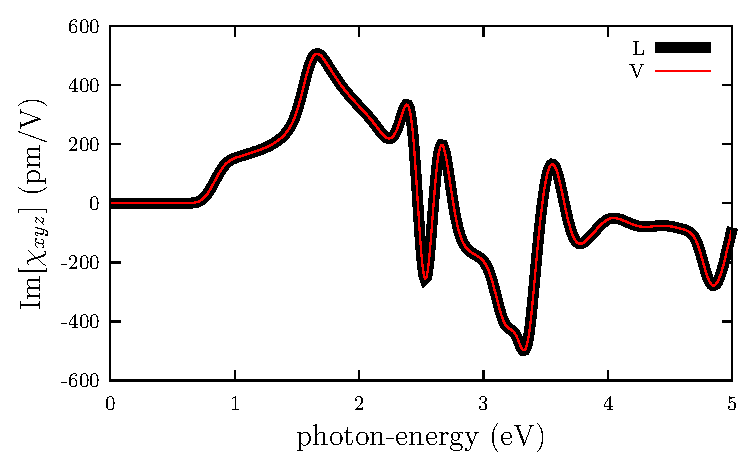
\includegraphics[scale=0.5]{plots/shg-bulk}
\end{center}
\caption{$\chi_{xyz}$ for GaAs, $E_{cut}=20$ Ha and $N_k=1661$. Both
  the length ($L$) and velocity ($V$) gauge results are shown.
The scissors shift is 1.051 eV.
}
\label{shg-bulk}
\end{figure}
\begin{figure}[ht]
\begin{center}
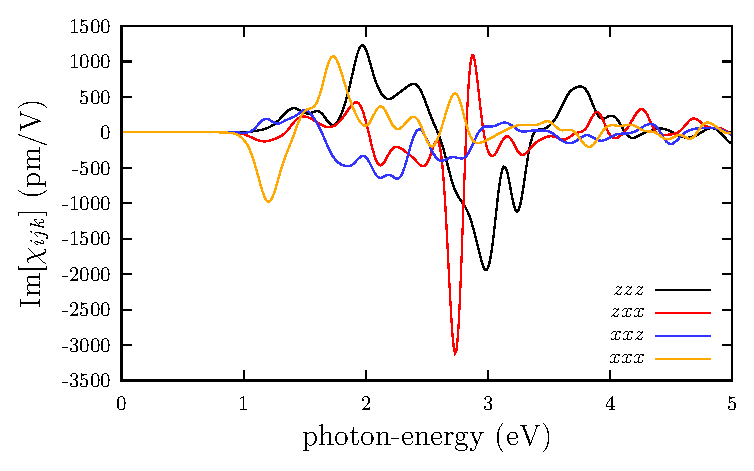
\includegraphics[scale=0.5]{plots/shg-surface}
\end{center}
\caption{Surface $\chi_{ijk}$ for all the allowed components of the
  si\_as\_6 example, $E_{cut}=5$ 
  Ha, $N_k=64$, and with a scissors shift of 0 eV. 
}
\label{shg-surface}
\end{figure}

\section{Surface} 
For an example copy from \verb=$TINIBA/examples/surface/nospin/si_as_6=:\\
\verb=setUpAbinit_si_as_6.in= and \verb=si_as_6.xyz=. This is a
Si(111)$1\times 1$:As surface with 4 layers of Si, one top and one bottom
layer of As. See results in \verb=si_as_6/res= and Fig.~\ref{shg-surface}.
